\lstset{
	backgroundcolor=\color{szary},
	frame=single,
	breaklines=true,
}

\chapter{Przebiegi odpowiedzi skokowych}

Wspomniana wcześniej funkcja \verb+Y=symulacja_obiektu_UppYppZpp(Upp,Zpp,time,t)+ ma za zadanie symulować zachowanie obiektu w przypadku skoku sterowania (argument \verb+Upp+) lub zakłócenia (argument \verb+Zpp+) od zera do podanej wartości. Zazwyczaj w obliczeniach używa się skoku sterowania następującego w dyskretnej chwili 0. Program MATLAB nie umożliwia jednak indeksowania od zera ani liczb ujemnych, w związku z czym funkcja pobudza obiekt skokiem dopiero w chwili $k=16$, a po wykonaniu całej symulacji obcina wektor wyjścia $Y$ tak, aby wyniki symulacji zgadzały się z powyższym założeniem.

Czas symulacji, tj. ilość dyskretnych chwil, w których liczona jest odpowiedź skokowa ustalone zostało na \verb+time=200+. Taka ilość próbek pozwala zaobserwować ustalenie się procesu (pod koniec symulacji wartości wyjścia są niemal identyczne).

Implementację funkcji przedstawia poniższy listing:

\begin{lstlisting}[style=customc,frame=single]
function Y=symulacja_obiektu_UppYppZpp(Upp,Zpp,time,t)

	%alokacja pamieci
	U=zeros(time+16,1);
	Y=zeros(time+16,1);
	Z=zeros(time+16,1);
	
	for k=16:time+16
	U(k)=Upp;
	Z(k)=Zpp;
	
	%skok wejscia lub zaklocenia w zaleznosci od parametru t
	if (t == 1)
		Y(k)=symulacja_obiektu7y(U(k-4),U(k-5),Z(k-1),...
		Z(k-2),Y(k-1),Y(k-2));
	end
	if (t == 2)
		Y(k)=symulacja_obiektu7y(0,0,Z(k-1),Z(k-2),...
		Y(k-1),Y(k-2));
		end
	end
	
	%obciecie pierwszych elementow wektora
	Y=Y(16:time+16,1);
end
\end{lstlisting}

\section{Tory wejście-wyjście oraz wejście-zakłócenie}
Kolejnym krokiem związanym z badaniem symulowanego obiektu jest zbadanie jego odpowiedzi skokowych na różne wartości skoków sterowania i zakłócenia. Zaczynając od punktu pracy i używając funkcji \verb+Y=symulacja_obiektu_UppYppZpp(Upp,Zpp,time,t)+ dokonano tej procedury, a wyniki symulacji przedstawiono na Rys.~\ref{osu} i \ref{osz}. 

Dokładne działanie obiektu jest nieznane, można jednak stwierdzić, że symulacja została przeprowadzona prawidłowo ze względu na widoczne w obu przypadkach opóźnienie.

Na podstawie tych wykresów można też uznać, że właściwości dynamiczne obiektu są liniowe, tzn. wartości odpowiedzi skokowych w stanie ustalonym są wprost proporcjonalne do skoków sterowania/zakłócenia, które je wywołały.

\begin{figure}
	\centering
	\caption{Charakterystyka dla skoku wartości sterowania}
	% This file was created by matlab2tikz.
%
\definecolor{mycolor1}{rgb}{0.00000,0.44700,0.74100}%
\definecolor{mycolor2}{rgb}{0.85000,0.32500,0.09800}%
\definecolor{mycolor3}{rgb}{0.92900,0.69400,0.12500}%
\definecolor{mycolor4}{rgb}{0.49400,0.18400,0.55600}%
\definecolor{mycolor5}{rgb}{0.46600,0.67400,0.18800}%
\definecolor{mycolor6}{rgb}{0.30100,0.74500,0.93300}%
\definecolor{mycolor7}{rgb}{0.63500,0.07800,0.18400}%
%
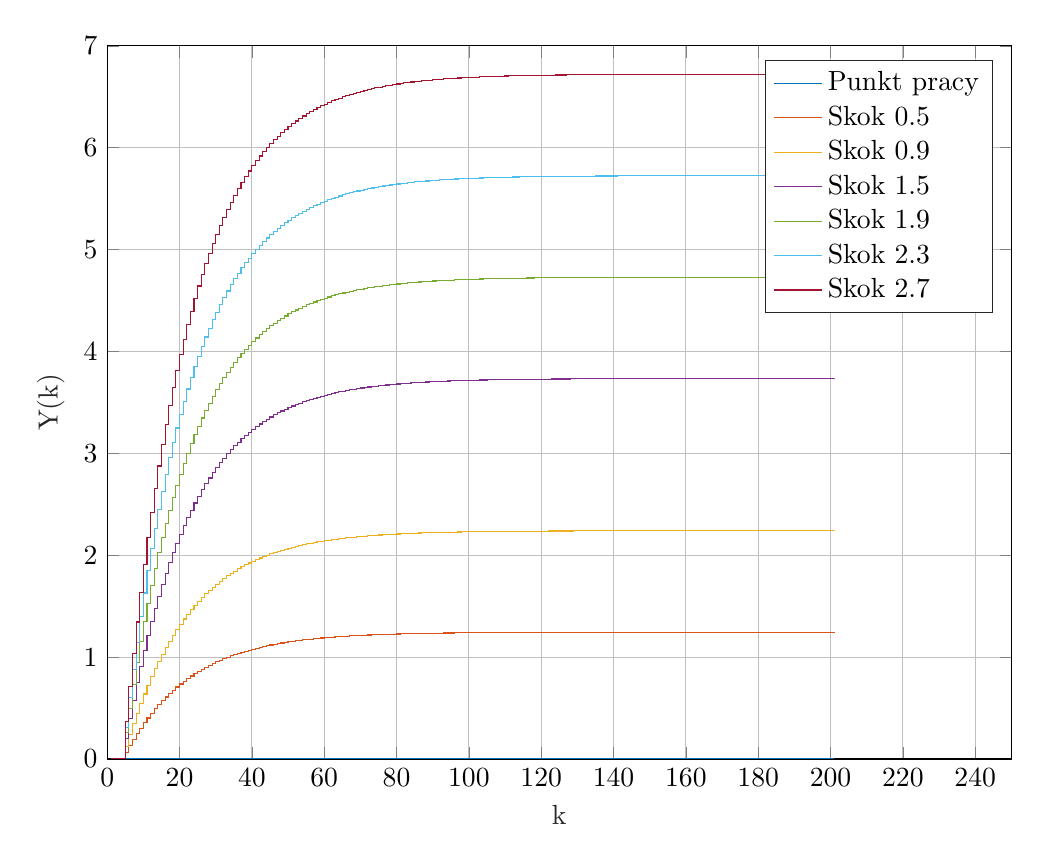
\begin{tikzpicture}

\begin{axis}[%
width=4.521in,
height=3.566in,
at={(0.758in,0.481in)},
scale only axis,
xmin=0,
xmax=250,
xlabel style={font=\color{white!15!black}},
xlabel={k},
ymin=0,
ymax=7,
ylabel style={font=\color{white!15!black}},
ylabel={Y(k)},
axis background/.style={fill=white},
title style={font=\bfseries},
title={ },
xmajorgrids,
ymajorgrids,
legend style={legend cell align=left, align=left, draw=white!15!black}
]
\addplot[const plot, color=mycolor1] table[row sep=crcr] {%
1	0\\
2	0\\
3	0\\
4	0\\
5	0\\
6	0\\
7	0\\
8	0\\
9	0\\
10	0\\
11	0\\
12	0\\
13	0\\
14	0\\
15	0\\
16	0\\
17	0\\
18	0\\
19	0\\
20	0\\
21	0\\
22	0\\
23	0\\
24	0\\
25	0\\
26	0\\
27	0\\
28	0\\
29	0\\
30	0\\
31	0\\
32	0\\
33	0\\
34	0\\
35	0\\
36	0\\
37	0\\
38	0\\
39	0\\
40	0\\
41	0\\
42	0\\
43	0\\
44	0\\
45	0\\
46	0\\
47	0\\
48	0\\
49	0\\
50	0\\
51	0\\
52	0\\
53	0\\
54	0\\
55	0\\
56	0\\
57	0\\
58	0\\
59	0\\
60	0\\
61	0\\
62	0\\
63	0\\
64	0\\
65	0\\
66	0\\
67	0\\
68	0\\
69	0\\
70	0\\
71	0\\
72	0\\
73	0\\
74	0\\
75	0\\
76	0\\
77	0\\
78	0\\
79	0\\
80	0\\
81	0\\
82	0\\
83	0\\
84	0\\
85	0\\
86	0\\
87	0\\
88	0\\
89	0\\
90	0\\
91	0\\
92	0\\
93	0\\
94	0\\
95	0\\
96	0\\
97	0\\
98	0\\
99	0\\
100	0\\
101	0\\
102	0\\
103	0\\
104	0\\
105	0\\
106	0\\
107	0\\
108	0\\
109	0\\
110	0\\
111	0\\
112	0\\
113	0\\
114	0\\
115	0\\
116	0\\
117	0\\
118	0\\
119	0\\
120	0\\
121	0\\
122	0\\
123	0\\
124	0\\
125	0\\
126	0\\
127	0\\
128	0\\
129	0\\
130	0\\
131	0\\
132	0\\
133	0\\
134	0\\
135	0\\
136	0\\
137	0\\
138	0\\
139	0\\
140	0\\
141	0\\
142	0\\
143	0\\
144	0\\
145	0\\
146	0\\
147	0\\
148	0\\
149	0\\
150	0\\
151	0\\
152	0\\
153	0\\
154	0\\
155	0\\
156	0\\
157	0\\
158	0\\
159	0\\
160	0\\
161	0\\
162	0\\
163	0\\
164	0\\
165	0\\
166	0\\
167	0\\
168	0\\
169	0\\
170	0\\
171	0\\
172	0\\
173	0\\
174	0\\
175	0\\
176	0\\
177	0\\
178	0\\
179	0\\
180	0\\
181	0\\
182	0\\
183	0\\
184	0\\
185	0\\
186	0\\
187	0\\
188	0\\
189	0\\
190	0\\
191	0\\
192	0\\
193	0\\
194	0\\
195	0\\
196	0\\
197	0\\
198	0\\
199	0\\
200	0\\
201	0\\
};
\addlegendentry{Punkt pracy}

\addplot[const plot, color=mycolor2] table[row sep=crcr] {%
1	0\\
2	0\\
3	0\\
4	0\\
5	0.06755\\
6	0.131446435\\
7	0.1918855133595\\
8	0.249053064198665\\
9	0.303125068556918\\
10	0.354268165429423\\
11	0.402640133624519\\
12	0.448390350381306\\
13	0.491660227677666\\
14	0.532583627145819\\
15	0.571287254495861\\
16	0.607891034328273\\
17	0.642508466194675\\
18	0.675246962742635\\
19	0.706208170755544\\
20	0.735488275872803\\
21	0.763178291749161\\
22	0.789364334385215\\
23	0.814127882334141\\
24	0.837546023462755\\
25	0.859691688918266\\
26	0.880633874925636\\
27	0.900437853014469\\
28	0.919165369248832\\
29	0.936874833008562\\
30	0.953621495846324\\
31	0.969457620921143\\
32	0.984432643486316\\
33	0.998593322887491\\
34	1.01198388650542\\
35	1.0246461660573\\
36	1.03661972665089\\
37	1.04794198896647\\
38	1.05864834492367\\
39	1.06877226717238\\
40	1.07834541273054\\
41	1.0873977210753\\
42	1.0959575069788\\
43	1.1040515483652\\
44	1.11170516945154\\
45	1.11894231942168\\
46	1.12578564686982\\
47	1.13225657023806\\
48	1.13837534446073\\
49	1.14416112401741\\
50	1.14963202258605\\
51	1.15480516947746\\
52	1.15969676302328\\
53	1.16432212108032\\
54	1.16869572880565\\
55	1.17283128384889\\
56	1.1767417391\\
57	1.18043934312422\\
58	1.18393567840809\\
59	1.18724169753463\\
60	1.19036775739892\\
61	1.19332365156979\\
62	1.19611864089748\\
63	1.19876148246192\\
64	1.20126045695113\\
65	1.20362339455459\\
66	1.20585769945176\\
67	1.2079703729717\\
68	1.2099680354956\\
69	1.21185694717039\\
70	1.21364302749749\\
71	1.21533187385792\\
72	1.21692877903116\\
73	1.21843874776229\\
74	1.21986651242914\\
75	1.22121654785801\\
76	1.22249308533437\\
77	1.22370012585196\\
78	1.22484145264178\\
79	1.22592064302002\\
80	1.22694107959177\\
81	1.22790596084565\\
82	1.22881831117229\\
83	1.22968099033806\\
84	1.23049670244353\\
85	1.23126800439469\\
86	1.2319973139135\\
87	1.23268691711257\\
88	1.23333897565789\\
89	1.23395553354192\\
90	1.23453852348807\\
91	1.23508977300691\\
92	1.23561101012272\\
93	1.23610386878857\\
94	1.23656989400663\\
95	1.23701054667001\\
96	1.23742720814097\\
97	1.23782118458008\\
98	1.2381937110398\\
99	1.23854595533517\\
100	1.23887902170399\\
101	1.23919395426768\\
102	1.23949174030385\\
103	1.23977331334072\\
104	1.24003955608311\\
105	1.24029130317919\\
106	1.24052934383664\\
107	1.24075442429641\\
108	1.24096725017174\\
109	1.24116848866005\\
110	1.2413587706342\\
111	1.24153869262011\\
112	1.2417088186666\\
113	1.24186968211351\\
114	1.24202178726351\\
115	1.242165610963\\
116	1.24230160409683\\
117	1.24243019300174\\
118	1.24255178080281\\
119	1.24266674867718\\
120	1.24277545704896\\
121	1.24287824671906\\
122	1.2429754399336\\
123	1.24306734139404\\
124	1.24315423921242\\
125	1.24323640581451\\
126	1.24331409879386\\
127	1.24338756171934\\
128	1.24345702489866\\
129	1.24352270610039\\
130	1.24358481123664\\
131	1.24364353500857\\
132	1.24369906151681\\
133	1.24375156483852\\
134	1.24380120957319\\
135	1.24384815135863\\
136	1.24389253735884\\
137	1.24393450672544\\
138	1.24397419103386\\
139	1.24401171469584\\
140	1.24404719534943\\
141	1.24408074422783\\
142	1.24411246650808\\
143	1.24414246164077\\
144	1.24417082366186\\
145	1.24419764148745\\
146	1.24422299919255\\
147	1.24424697627463\\
148	1.24426964790287\\
149	1.24429108515383\\
150	1.24431135523423\\
151	1.24433052169166\\
152	1.24434864461385\\
153	1.24436578081698\\
154	1.24438198402383\\
155	1.24439730503221\\
156	1.24441179187418\\
157	1.24442548996669\\
158	1.2444384422539\\
159	1.24445068934185\\
160	1.24446226962575\\
161	1.24447321941035\\
162	1.24448357302374\\
163	1.24449336292502\\
164	1.24450261980601\\
165	1.24451137268747\\
166	1.24451964901012\\
167	1.24452747472065\\
168	1.24453487435305\\
169	1.24454187110553\\
170	1.24454848691327\\
171	1.24455474251714\\
172	1.24456065752879\\
173	1.24456625049207\\
174	1.24457153894121\\
175	1.24457653945576\\
176	1.24458126771259\\
177	1.24458573853502\\
178	1.24458996593931\\
179	1.24459396317859\\
180	1.24459774278441\\
181	1.24460131660602\\
182	1.24460469584755\\
183	1.24460789110307\\
184	1.24461091238989\\
185	1.2446137691799\\
186	1.24461647042927\\
187	1.24461902460656\\
188	1.24462143971926\\
189	1.24462372333886\\
190	1.24462588262464\\
191	1.24462792434605\\
192	1.24462985490401\\
193	1.24463168035091\\
194	1.24463340640963\\
195	1.24463503849145\\
196	1.24463658171302\\
197	1.24463804091244\\
198	1.24463942066436\\
199	1.24464072529437\\
200	1.24464195889257\\
201	1.24464312532635\\
};
\addlegendentry{Skok 0.5}

\addplot[const plot, color=mycolor3] table[row sep=crcr] {%
1	0\\
2	0\\
3	0\\
4	0\\
5	0.12159\\
6	0.236603583\\
7	0.3453939240471\\
8	0.448295515557597\\
9	0.545625123402452\\
10	0.637682697772962\\
11	0.724752240524135\\
12	0.807102630686351\\
13	0.884988409819798\\
14	0.958650528862473\\
15	1.02831705809255\\
16	1.09420386179089\\
17	1.15651523915042\\
18	1.21544453293674\\
19	1.27117470735998\\
20	1.32387889657105\\
21	1.37372092514849\\
22	1.42085580189339\\
23	1.46543018820146\\
24	1.50758284223297\\
25	1.54744504005289\\
26	1.58514097486616\\
27	1.62078813542606\\
28	1.65449766464791\\
29	1.68637469941543\\
30	1.7165186925234\\
31	1.74502371765808\\
32	1.77197875827539\\
33	1.79746798119751\\
34	1.82157099570978\\
35	1.84436309890317\\
36	1.86591550797162\\
37	1.88629558013967\\
38	1.90556702086263\\
39	1.92379008091031\\
40	1.94102174291501\\
41	1.95731589793558\\
42	1.97272351256188\\
43	1.9872927870574\\
44	2.00106930501281\\
45	2.01409617495906\\
46	2.02641416436572\\
47	2.03806182642855\\
48	2.04907562002934\\
49	2.05949002323138\\
50	2.06933764065494\\
51	2.07864930505948\\
52	2.08745417344196\\
53	2.09577981794462\\
54	2.10365231185022\\
55	2.11109631092804\\
56	2.11813513038005\\
57	2.12479081762365\\
58	2.13108422113461\\
59	2.13703505556238\\
60	2.1426619633181\\
61	2.14798257282567\\
62	2.15301355361552\\
63	2.15777066843151\\
64	2.16226882251209\\
65	2.16652211019831\\
66	2.17054385901322\\
67	2.17434667134911\\
68	2.17794246389214\\
69	2.18134250490675\\
70	2.18455744949553\\
71	2.18759737294432\\
72	2.19047180225614\\
73	2.19318974597218\\
74	2.1957597223725\\
75	2.19818978614448\\
76	2.20048755360192\\
77	2.20266022653358\\
78	2.20471461475526\\
79	2.20665715743609\\
80	2.20849394326524\\
81	2.21023072952222\\
82	2.21187296011017\\
83	2.21342578260856\\
84	2.2148940643984\\
85	2.2162824079105\\
86	2.21759516504435\\
87	2.21883645080267\\
88	2.22001015618426\\
89	2.22111996037551\\
90	2.22216934227859\\
91	2.2231615914125\\
92	2.22409981822096\\
93	2.22498696381947\\
94	2.22582580921199\\
95	2.22661898400607\\
96	2.2273689746538\\
97	2.22807813224421\\
98	2.2287486798717\\
99	2.22938271960336\\
100	2.22998223906724\\
101	2.23054911768188\\
102	2.231085132547\\
103	2.23159196401336\\
104	2.23207120094965\\
105	2.2325243457226\\
106	2.23295281890603\\
107	2.2333579637336\\
108	2.2337410503092\\
109	2.23410327958815\\
110	2.23444578714163\\
111	2.23476964671627\\
112	2.23507587359996\\
113	2.23536542780439\\
114	2.23563921707439\\
115	2.23589809973347\\
116	2.23614288737436\\
117	2.23637434740319\\
118	2.23659320544512\\
119	2.23680014761899\\
120	2.23699582268819\\
121	2.23718084409438\\
122	2.23735579188055\\
123	2.23752121450934\\
124	2.23767763058241\\
125	2.23782553046617\\
126	2.23796537782902\\
127	2.23809761109488\\
128	2.23822264481766\\
129	2.23834087098076\\
130	2.23845266022601\\
131	2.2385583630155\\
132	2.23865831073032\\
133	2.2387528167094\\
134	2.23884217723181\\
135	2.23892667244559\\
136	2.23900656724597\\
137	2.23908211210586\\
138	2.23915354386102\\
139	2.23922108645258\\
140	2.23928495162904\\
141	2.23934533961016\\
142	2.23940243971461\\
143	2.23945643095345\\
144	2.23950748259142\\
145	2.23955575467749\\
146	2.23960139854666\\
147	2.2396445572944\\
148	2.23968536622525\\
149	2.23972395327697\\
150	2.23976043942168\\
151	2.23979493904507\\
152	2.23982756030501\\
153	2.23985840547063\\
154	2.23988757124296\\
155	2.23991514905804\\
156	2.23994122537359\\
157	2.23996588194011\\
158	2.23998919605709\\
159	2.2400112408154\\
160	2.24003208532642\\
161	2.24005179493869\\
162	2.2400704314428\\
163	2.24008805326511\\
164	2.24010471565087\\
165	2.2401204708375\\
166	2.24013536821828\\
167	2.24014945449724\\
168	2.24016277383556\\
169	2.24017536799002\\
170	2.24018727644394\\
171	2.24019853653092\\
172	2.24020918355189\\
173	2.24021925088579\\
174	2.24022877009424\\
175	2.24023777102043\\
176	2.24024628188272\\
177	2.2402543293631\\
178	2.24026193869082\\
179	2.24026913372153\\
180	2.240275937012\\
181	2.2402823698909\\
182	2.24028845252564\\
183	2.24029420398558\\
184	2.24029964230186\\
185	2.24030478452387\\
186	2.24030964677273\\
187	2.24031424429187\\
188	2.24031859149472\\
189	2.24032270201001\\
190	2.24032658872439\\
191	2.24033026382294\\
192	2.24033373882726\\
193	2.24033702463169\\
194	2.24034013153738\\
195	2.24034306928465\\
196	2.24034584708349\\
197	2.24034847364243\\
198	2.24035095719589\\
199	2.24035330552993\\
200	2.24035552600669\\
201	2.24035762558749\\
};
\addlegendentry{Skok 0.9}

\addplot[const plot, color=mycolor4] table[row sep=crcr] {%
1	0\\
2	0\\
3	0\\
4	0\\
5	0.20265\\
6	0.394339305\\
7	0.5756565400785\\
8	0.747159192595996\\
9	0.909375205670754\\
10	1.06280449628827\\
11	1.20792040087356\\
12	1.34517105114392\\
13	1.474980683033\\
14	1.59775088143746\\
15	1.71386176348758\\
16	1.82367310298482\\
17	1.92752539858402\\
18	2.0257408882279\\
19	2.11862451226663\\
20	2.20646482761841\\
21	2.28953487524748\\
22	2.36809300315564\\
23	2.44238364700242\\
24	2.51263807038826\\
25	2.57907506675479\\
26	2.6419016247769\\
27	2.7013135590434\\
28	2.75749610774649\\
29	2.81062449902568\\
30	2.86086448753897\\
31	2.90837286276343\\
32	2.95329793045894\\
33	2.99577996866247\\
34	3.03595165951625\\
35	3.0739384981719\\
36	3.10985917995266\\
37	3.14382596689941\\
38	3.175945034771\\
39	3.20631680151713\\
40	3.23503623819163\\
41	3.26219316322591\\
42	3.28787252093641\\
43	3.3121546450956\\
44	3.33511550835462\\
45	3.35682695826503\\
46	3.37735694060946\\
47	3.39676971071418\\
48	3.41512603338217\\
49	3.43248337205223\\
50	3.44889606775816\\
51	3.46441550843239\\
52	3.47909028906985\\
53	3.49296636324095\\
54	3.50608718641696\\
55	3.51849385154666\\
56	3.53022521730002\\
57	3.54131802937267\\
58	3.55180703522428\\
59	3.56172509260389\\
60	3.57110327219675\\
61	3.57997095470937\\
62	3.58835592269245\\
63	3.59628444738577\\
64	3.6037813708534\\
65	3.61087018366378\\
66	3.61757309835529\\
67	3.6239111189151\\
68	3.62990410648682\\
69	3.63557084151117\\
70	3.64092908249247\\
71	3.64599562157378\\
72	3.65078633709348\\
73	3.65531624328688\\
74	3.65959953728741\\
75	3.66364964357404\\
76	3.66747925600312\\
77	3.67110037755588\\
78	3.67452435792536\\
79	3.67776192906007\\
80	3.68082323877532\\
81	3.68371788253695\\
82	3.68645493351687\\
83	3.68904297101419\\
84	3.69149010733058\\
85	3.69380401318408\\
86	3.6959919417405\\
87	3.6980607513377\\
88	3.70001692697368\\
89	3.70186660062575\\
90	3.70361557046422\\
91	3.70526931902073\\
92	3.70683303036817\\
93	3.7083116063657\\
94	3.70970968201989\\
95	3.71103164001003\\
96	3.7122816244229\\
97	3.71346355374025\\
98	3.71458113311939\\
99	3.71563786600551\\
100	3.71663706511196\\
101	3.71758186280304\\
102	3.71847522091156\\
103	3.71931994002216\\
104	3.72011866824932\\
105	3.72087390953756\\
106	3.72158803150993\\
107	3.72226327288922\\
108	3.72290175051523\\
109	3.72350546598014\\
110	3.7240763119026\\
111	3.72461607786034\\
112	3.72512645599981\\
113	3.72560904634053\\
114	3.72606536179054\\
115	3.726496832889\\
116	3.72690481229049\\
117	3.72729057900521\\
118	3.72765534240843\\
119	3.72800024603155\\
120	3.72832637114687\\
121	3.72863474015719\\
122	3.7289263198008\\
123	3.72920202418213\\
124	3.72946271763725\\
125	3.72970921744352\\
126	3.72994229638159\\
127	3.73016268515804\\
128	3.73037107469599\\
129	3.73056811830117\\
130	3.73075443370991\\
131	3.73093060502573\\
132	3.73109718455043\\
133	3.73125469451556\\
134	3.73140362871959\\
135	3.73154445407588\\
136	3.73167761207652\\
137	3.73180352017633\\
138	3.7319225731016\\
139	3.73203514408752\\
140	3.7321415860483\\
141	3.7322422326835\\
142	3.73233739952424\\
143	3.73242738492232\\
144	3.73251247098559\\
145	3.73259292446237\\
146	3.73266899757766\\
147	3.73274092882389\\
148	3.73280894370864\\
149	3.73287325546151\\
150	3.73293406570269\\
151	3.73299156507501\\
152	3.73304593384158\\
153	3.73309734245096\\
154	3.73314595207151\\
155	3.73319191509663\\
156	3.73323537562256\\
157	3.73327646990009\\
158	3.73331532676173\\
159	3.73335206802558\\
160	3.73338680887728\\
161	3.73341965823106\\
162	3.73345071907125\\
163	3.73348008877508\\
164	3.73350785941803\\
165	3.73353411806241\\
166	3.73355894703038\\
167	3.73358242416197\\
168	3.73360462305917\\
169	3.73362561331661\\
170	3.73364546073981\\
171	3.73366422755144\\
172	3.73368197258639\\
173	3.73369875147623\\
174	3.73371461682365\\
175	3.7337296183673\\
176	3.73374380313778\\
177	3.73375721560508\\
178	3.73376989781795\\
179	3.73378188953579\\
180	3.73379322835324\\
181	3.73380394981808\\
182	3.73381408754264\\
183	3.73382367330922\\
184	3.73383273716968\\
185	3.73384130753969\\
186	3.7338494112878\\
187	3.73385707381969\\
188	3.73386431915778\\
189	3.73387117001659\\
190	3.7338776478739\\
191	3.73388377303815\\
192	3.73388956471202\\
193	3.73389504105273\\
194	3.73390021922889\\
195	3.73390511547434\\
196	3.73390974513906\\
197	3.73391412273731\\
198	3.73391826199307\\
199	3.73392217588312\\
200	3.73392587667772\\
201	3.73392937597906\\
};
\addlegendentry{Skok 1.5}

\addplot[const plot, color=mycolor5] table[row sep=crcr] {%
1	0\\
2	0\\
3	0\\
4	0\\
5	0.25669\\
6	0.499496453\\
7	0.7291649507661\\
8	0.946401643954927\\
9	1.15187526051629\\
10	1.34621902863181\\
11	1.53003250777317\\
12	1.70388333144896\\
13	1.86830886517513\\
14	2.02381778315411\\
15	2.17089156708427\\
16	2.30998593044744\\
17	2.44153217153976\\
18	2.56593845842201\\
19	2.68359104887107\\
20	2.79485544831666\\
21	2.90007750864682\\
22	2.99958447066382\\
23	3.09368595286974\\
24	3.18267488915848\\
25	3.26682841788942\\
26	3.34640872471743\\
27	3.42166384145499\\
28	3.49282840314557\\
29	3.56012436543255\\
30	3.62376168421604\\
31	3.68393895950036\\
32	3.74084404524802\\
33	3.79465462697249\\
34	3.84553876872061\\
35	3.89365543101776\\
36	3.93915496127339\\
37	3.98217955807261\\
38	4.02286371070996\\
39	4.06133461525506\\
40	4.09771256837609\\
41	4.13211134008619\\
42	4.16463852651948\\
43	4.1953958837878\\
44	4.22447964391589\\
45	4.25198081380241\\
46	4.27798545810536\\
47	4.30257496690467\\
48	4.32582630895079\\
49	4.3478122712662\\
50	4.36860168582704\\
51	4.3882596440144\\
52	4.40684769948852\\
53	4.42442406010524\\
54	4.44104376946152\\
55	4.4567588786258\\
56	4.47161860858005\\
57	4.48566950387207\\
58	4.49895557795078\\
59	4.51151845063161\\
60	4.52339747811591\\
61	4.53462987596521\\
62	4.54525083541045\\
63	4.55529363335532\\
64	4.56478973641431\\
65	4.57376889930745\\
66	4.5822592579167\\
67	4.59028741729245\\
68	4.5978785348833\\
69	4.60505639924748\\
70	4.61184350449045\\
71	4.6182611206601\\
72	4.62432936031839\\
73	4.63006724149669\\
74	4.63549274723069\\
75	4.64062288186041\\
76	4.64547372427058\\
77	4.6500604782374\\
78	4.65439752003874\\
79	4.65849844347604\\
80	4.66237610244868\\
81	4.66604265121341\\
82	4.66950958245465\\
83	4.67278776328458\\
84	4.67588746928534\\
85	4.67881841669977\\
86	4.68158979287124\\
87	4.68421028502768\\
88	4.68668810749993\\
89	4.68903102745922\\
90	4.6912463892546\\
91	4.69334113742619\\
92	4.69532183846628\\
93	4.69719470139648\\
94	4.69896559722512\\
95	4.70064007734596\\
96	4.7022233909356\\
97	4.70372050140424\\
98	4.70513610195116\\
99	4.70647463027357\\
100	4.70774028247507\\
101	4.70893702621711\\
102	4.71006861315456\\
103	4.71113859069466\\
104	4.71215031311572\\
105	4.71310695208084\\
106	4.71401150657917\\
107	4.71486681232626\\
108	4.71567555065255\\
109	4.7164402569081\\
110	4.71716332840988\\
111	4.71784703195635\\
112	4.71849351093302\\
113	4.71910479203126\\
114	4.71968279160127\\
115	4.72022932165933\\
116	4.72074609556787\\
117	4.72123473340652\\
118	4.7216967670506\\
119	4.72213364497322\\
120	4.72254673678597\\
121	4.72293733753237\\
122	4.72330667174761\\
123	4.7236558972973\\
124	4.72398610900712\\
125	4.72429834209506\\
126	4.72459357541662\\
127	4.72487273453345\\
128	4.72513669461486\\
129	4.72538628318142\\
130	4.72562228269916\\
131	4.72584543303253\\
132	4.72605643376381\\
133	4.72625594638632\\
134	4.72644459637808\\
135	4.72662297516272\\
136	4.72679164196353\\
137	4.72695112555662\\
138	4.72710192592863\\
139	4.72724451584413\\
140	4.72737934232777\\
141	4.7275068280657\\
142	4.72762737273063\\
143	4.72774135423486\\
144	4.72784912991501\\
145	4.72795103765226\\
146	4.72804739693162\\
147	4.72813850984352\\
148	4.72822466203086\\
149	4.7283061235845\\
150	4.72838314988999\\
151	4.72845598242826\\
152	4.72852484953258\\
153	4.72858996710446\\
154	4.72865153929048\\
155	4.7287097591223\\
156	4.72876480912181\\
157	4.72881686187335\\
158	4.72886608056475\\
159	4.72891261949897\\
160	4.72895662457778\\
161	4.72899823375924\\
162	4.72903757749015\\
163	4.72907477911501\\
164	4.72910995526274\\
165	4.72914321621229\\
166	4.72917466623838\\
167	4.7292044039384\\
168	4.72923252254151\\
169	4.72925911020094\\
170	4.72928425027033\\
171	4.72930802156505\\
172	4.72933049860932\\
173	4.72935175186979\\
174	4.72937184797651\\
175	4.7293908499318\\
176	4.72940881730775\\
177	4.72942580643299\\
178	4.7294418705693\\
179	4.72945706007856\\
180	4.72947142258067\\
181	4.72948500310279\\
182	4.72949784422057\\
183	4.72950998619157\\
184	4.72952146708148\\
185	4.7295323228835\\
186	4.72954258763111\\
187	4.72955229350484\\
188	4.72956147093309\\
189	4.72957014868757\\
190	4.72957835397351\\
191	4.72958611251488\\
192	4.72959344863513\\
193	4.72960038533336\\
194	4.72960694435649\\
195	4.7296131462674\\
196	4.72961901050938\\
197	4.72962455546716\\
198	4.72962979852446\\
199	4.72963475611853\\
200	4.7296394437917\\
201	4.72964387624005\\
};
\addlegendentry{Skok 1.9}

\addplot[const plot, color=mycolor6] table[row sep=crcr] {%
1	0\\
2	0\\
3	0\\
4	0\\
5	0.31073\\
6	0.604653601\\
7	0.8826733614537\\
8	1.14564409531386\\
9	1.39437531536182\\
10	1.62963356097535\\
11	1.85214461467279\\
12	2.06259561175401\\
13	2.26163704731726\\
14	2.44988468487076\\
15	2.62792137068096\\
16	2.79629875791006\\
17	2.95553894449551\\
18	3.10613602861613\\
19	3.24855758547551\\
20	3.38324606901491\\
21	3.51062014204616\\
22	3.63107593817201\\
23	3.74498825873707\\
24	3.8527117079287\\
25	3.95458176902405\\
26	4.05091582465795\\
27	4.14201412386659\\
28	4.22816069854466\\
29	4.30962423183942\\
30	4.38665888089313\\
31	4.4595050562373\\
32	4.5283901600371\\
33	4.59352928528251\\
34	4.65512587792498\\
35	4.71337236386363\\
36	4.76845074259413\\
37	4.82053314924581\\
38	4.86978238664893\\
39	4.91635242899299\\
40	4.96038889856055\\
41	5.00202951694646\\
42	5.04140453210255\\
43	5.07863712247998\\
44	5.11384377947714\\
45	5.14713466933977\\
46	5.17861397560123\\
47	5.20838022309513\\
48	5.23652658451938\\
49	5.26314117048013\\
50	5.28830730389589\\
51	5.31210377959638\\
52	5.33460510990715\\
53	5.3558817569695\\
54	5.37600035250605\\
55	5.39502390570492\\
56	5.41301199986006\\
57	5.43002097837146\\
58	5.44610412067726\\
59	5.46131180865933\\
60	5.47569168403505\\
61	5.48928879722106\\
62	5.50214574812846\\
63	5.51430281932488\\
64	5.52579810197524\\
65	5.53666761495115\\
66	5.54694541747814\\
67	5.55666371566983\\
68	5.56585296327981\\
69	5.57454195698382\\
70	5.58275792648848\\
71	5.59052661974648\\
72	5.59787238354336\\
73	5.60481823970656\\
74	5.61138595717405\\
75	5.61759612014687\\
76	5.62346819253813\\
77	5.62902057891903\\
78	5.63427068215222\\
79	5.63923495789212\\
80	5.64392896612216\\
81	5.64836741988999\\
82	5.65256423139254\\
83	5.65653255555509\\
84	5.66028483124022\\
85	5.66383282021558\\
86	5.66718764400209\\
87	5.67035981871779\\
88	5.6733592880263\\
89	5.67619545429281\\
90	5.67887720804512\\
91	5.68141295583178\\
92	5.68381064656452\\
93	5.68607779642739\\
94	5.68822151243049\\
95	5.69024851468203\\
96	5.69216515744843\\
97	5.69397744906837\\
98	5.69569107078306\\
99	5.69731139454176\\
100	5.69884349983832\\
101	5.70029218963131\\
102	5.7016620053977\\
103	5.70295724136729\\
104	5.70418195798227\\
105	5.70533999462425\\
106	5.70643498164855\\
107	5.70747035176346\\
108	5.70844935079001\\
109	5.70937504783621\\
110	5.71025034491732\\
111	5.71107798605251\\
112	5.71186056586637\\
113	5.71260053772213\\
114	5.71330022141215\\
115	5.7139618104298\\
116	5.7145873788454\\
117	5.71517888780798\\
118	5.71573819169291\\
119	5.71626704391502\\
120	5.71676710242519\\
121	5.71723993490767\\
122	5.71768702369455\\
123	5.71810977041258\\
124	5.7185095003771\\
125	5.71888746674671\\
126	5.71924485445176\\
127	5.71958278390897\\
128	5.71990231453383\\
129	5.72020444806178\\
130	5.72049013168852\\
131	5.72076026103943\\
132	5.7210156829773\\
133	5.72125719825718\\
134	5.72148556403668\\
135	5.72170149624966\\
136	5.72190567185064\\
137	5.72209873093701\\
138	5.72228127875576\\
139	5.72245388760083\\
140	5.72261709860735\\
141	5.722771423448\\
142	5.72291734593712\\
143	5.72305532354751\\
144	5.72318578884453\\
145	5.72330915084226\\
146	5.72342579628569\\
147	5.72353609086326\\
148	5.7236403803532\\
149	5.7237389917076\\
150	5.72383223407741\\
151	5.72392039978163\\
152	5.7240037652237\\
153	5.72408259175808\\
154	5.72415712650959\\
155	5.72422760314811\\
156	5.72429424262121\\
157	5.72435725384675\\
158	5.72441683436793\\
159	5.7244731709725\\
160	5.72452644027844\\
161	5.72457680928757\\
162	5.72462443590919\\
163	5.72466946945508\\
164	5.72471205110759\\
165	5.72475231436231\\
166	5.72479038544653\\
167	5.72482638371497\\
168	5.724860422024\\
169	5.72489260708542\\
170	5.72492303980099\\
171	5.72495181557882\\
172	5.72497902463241\\
173	5.72500475226351\\
174	5.72502907912954\\
175	5.72505208149647\\
176	5.72507383147788\\
177	5.72509439726107\\
178	5.72511384332081\\
179	5.7251322306215\\
180	5.72514961680826\\
181	5.72516605638767\\
182	5.72518160089867\\
183	5.72519629907409\\
184	5.72521019699346\\
185	5.72522333822748\\
186	5.72523576397459\\
187	5.72524751319015\\
188	5.72525862270856\\
189	5.72526912735872\\
190	5.72527906007327\\
191	5.72528845199178\\
192	5.7252973325584\\
193	5.72530572961415\\
194	5.72531366948425\\
195	5.72532117706061\\
196	5.72532827587986\\
197	5.72533498819717\\
198	5.725341335056\\
199	5.72534733635408\\
200	5.72535301090581\\
201	5.72535837650118\\
};
\addlegendentry{Skok 2.3}

\addplot[const plot, color=mycolor7] table[row sep=crcr] {%
1	0\\
2	0\\
3	0\\
4	0\\
5	0.36477\\
6	0.709810749\\
7	1.0361817721413\\
8	1.34488654667279\\
9	1.63687537020736\\
10	1.91304809331889\\
11	2.17425672157241\\
12	2.42130789205905\\
13	2.65496522945939\\
14	2.87595158658742\\
15	3.08495117427765\\
16	3.28261158537267\\
17	3.46954571745124\\
18	3.64633359881023\\
19	3.81352412207993\\
20	3.97163668971314\\
21	4.12116277544547\\
22	4.26256740568016\\
23	4.39629056460436\\
24	4.52274852669888\\
25	4.64233512015864\\
26	4.75542292459844\\
27	4.86236440627814\\
28	4.9634929939437\\
29	5.05912409824624\\
30	5.14955607757016\\
31	5.23507115297418\\
32	5.31593627482612\\
33	5.39240394359247\\
34	5.46471298712928\\
35	5.53308929670944\\
36	5.5977465239148\\
37	5.65888674041896\\
38	5.71670106258783\\
39	5.77137024273087\\
40	5.82306522874496\\
41	5.87194769380667\\
42	5.91817053768557\\
43	5.96187836117212\\
44	6.00320791503836\\
45	6.0422885248771\\
46	6.07924249309707\\
47	6.11418547928556\\
48	6.14722686008795\\
49	6.17847006969405\\
50	6.20801292196472\\
51	6.23594791517834\\
52	6.26236252032577\\
53	6.28733945383375\\
54	6.31095693555056\\
55	6.33328893278403\\
56	6.35440539114006\\
57	6.37437245287084\\
58	6.39325266340374\\
59	6.41110516668704\\
60	6.4279858899542\\
61	6.44394771847691\\
62	6.45904066084646\\
63	6.47331200529444\\
64	6.48680646753616\\
65	6.49956633059485\\
66	6.51163157703957\\
67	6.52304001404722\\
68	6.53382739167632\\
69	6.54402751472016\\
70	6.5536723484865\\
71	6.56279211883285\\
72	6.57141540676832\\
73	6.57956923791643\\
74	6.58727916711739\\
75	6.59456935843332\\
76	6.60146266080566\\
77	6.60798067960063\\
78	6.61414384426568\\
79	6.61997147230817\\
80	6.62548182979562\\
81	6.63069218856655\\
82	6.63561888033042\\
83	6.64027734782558\\
84	6.64468219319509\\
85	6.64884722373139\\
86	6.65278549513295\\
87	6.6565093524079\\
88	6.66003046855267\\
89	6.6633598811264\\
90	6.66650802683563\\
91	6.66948477423736\\
92	6.67229945466275\\
93	6.67496089145829\\
94	6.67747742763584\\
95	6.67985695201808\\
96	6.68210692396126\\
97	6.68423439673249\\
98	6.68624603961494\\
99	6.68814815880994\\
100	6.68994671720156\\
101	6.6916473530455\\
102	6.69325539764083\\
103	6.69477589203991\\
104	6.6962136028488\\
105	6.69757303716764\\
106	6.69885845671791\\
107	6.70007389120062\\
108	6.70122315092744\\
109	6.70230983876428\\
110	6.70333736142471\\
111	6.70430894014863\\
112	6.70522762079968\\
113	6.70609628341297\\
114	6.70691765122299\\
115	6.70769429920022\\
116	6.70842866212289\\
117	6.70912304220939\\
118	6.70977961633518\\
119	6.71040044285679\\
120	6.71098746806438\\
121	6.71154253228295\\
122	6.71206737564146\\
123	6.71256364352784\\
124	6.71303289174707\\
125	6.71347659139835\\
126	6.71389613348689\\
127	6.71429283328449\\
128	6.71466793445281\\
129	6.71502261294214\\
130	6.71535798067787\\
131	6.71567508904634\\
132	6.7159749321908\\
133	6.71625845012805\\
134	6.71652653169529\\
135	6.71678001733661\\
136	6.71701970173776\\
137	6.71724633631742\\
138	6.71746063158291\\
139	6.71766325935756\\
140	6.71785485488696\\
141	6.71803601883032\\
142	6.71820731914365\\
143	6.71836929286019\\
144	6.71852244777409\\
145	6.71866726403228\\
146	6.7188041956398\\
147	6.71893367188303\\
148	6.71905609867556\\
149	6.71917185983073\\
150	6.71928131826486\\
151	6.71938481713503\\
152	6.71948268091485\\
153	6.71957521641174\\
154	6.71966271372872\\
155	6.71974544717394\\
156	6.71982367612062\\
157	6.71989764582017\\
158	6.71996758817111\\
159	6.72003372244605\\
160	6.72009625597911\\
161	6.72015538481592\\
162	6.72021129432825\\
163	6.72026415979516\\
164	6.72031414695246\\
165	6.72036141251235\\
166	6.72040610465469\\
167	6.72044836349156\\
168	6.72048832150651\\
169	6.72052610396991\\
170	6.72056182933167\\
171	6.7205956095926\\
172	6.7206275506555\\
173	6.72065775265723\\
174	6.72068631028257\\
175	6.72071331306114\\
176	6.72073884564801\\
177	6.72076298808915\\
178	6.72078581607232\\
179	6.72080740116443\\
180	6.72082781103585\\
181	6.72084710967256\\
182	6.72086535757677\\
183	6.72088261195661\\
184	6.72089892690544\\
185	6.72091435357146\\
186	6.72092894031807\\
187	6.72094273287547\\
188	6.72095577448403\\
189	6.72096810602988\\
190	6.72097976617305\\
191	6.72099079146869\\
192	6.72100121648167\\
193	6.72101107389494\\
194	6.72102039461202\\
195	6.72102920785382\\
196	6.72103754125033\\
197	6.72104542092717\\
198	6.72105287158754\\
199	6.72105991658964\\
200	6.72106657801992\\
201	6.72107287676232\\
};
\addlegendentry{Skok 2.7}

\end{axis}
\end{tikzpicture}%
	\label{osu}
\end{figure}

\begin{figure}
	\centering
	\caption{Charakterystyka dla skoku wartości zakłócenia}
	% This file was created by matlab2tikz.
%
\definecolor{mycolor1}{rgb}{0.00000,0.44700,0.74100}%
\definecolor{mycolor2}{rgb}{0.85000,0.32500,0.09800}%
\definecolor{mycolor3}{rgb}{0.92900,0.69400,0.12500}%
\definecolor{mycolor4}{rgb}{0.49400,0.18400,0.55600}%
\definecolor{mycolor5}{rgb}{0.46600,0.67400,0.18800}%
\definecolor{mycolor6}{rgb}{0.30100,0.74500,0.93300}%
\definecolor{mycolor7}{rgb}{0.63500,0.07800,0.18400}%
%
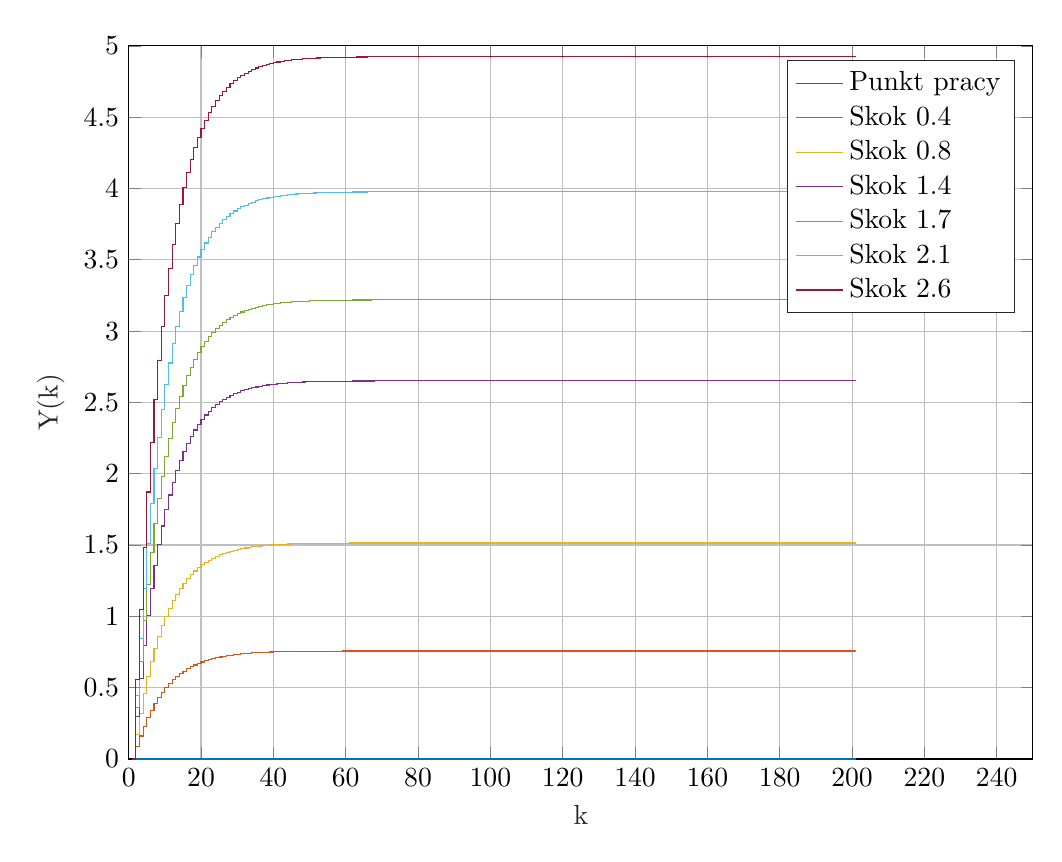
\begin{tikzpicture}

\begin{axis}[%
width=4.521in,
height=3.566in,
at={(0.758in,0.481in)},
scale only axis,
xmin=0,
xmax=250,
xlabel style={font=\color{white!15!black}},
xlabel={k},
ymin=0,
ymax=5,
ylabel style={font=\color{white!15!black}},
ylabel={Y(k)},
axis background/.style={fill=white},
title style={font=\bfseries},
title={ },
xmajorgrids,
ymajorgrids,
legend style={legend cell align=left, align=left, draw=white!15!black}
]
\addplot[const plot, color=mycolor1] table[row sep=crcr] {%
1	0\\
2	0\\
3	0\\
4	0\\
5	0\\
6	0\\
7	0\\
8	0\\
9	0\\
10	0\\
11	0\\
12	0\\
13	0\\
14	0\\
15	0\\
16	0\\
17	0\\
18	0\\
19	0\\
20	0\\
21	0\\
22	0\\
23	0\\
24	0\\
25	0\\
26	0\\
27	0\\
28	0\\
29	0\\
30	0\\
31	0\\
32	0\\
33	0\\
34	0\\
35	0\\
36	0\\
37	0\\
38	0\\
39	0\\
40	0\\
41	0\\
42	0\\
43	0\\
44	0\\
45	0\\
46	0\\
47	0\\
48	0\\
49	0\\
50	0\\
51	0\\
52	0\\
53	0\\
54	0\\
55	0\\
56	0\\
57	0\\
58	0\\
59	0\\
60	0\\
61	0\\
62	0\\
63	0\\
64	0\\
65	0\\
66	0\\
67	0\\
68	0\\
69	0\\
70	0\\
71	0\\
72	0\\
73	0\\
74	0\\
75	0\\
76	0\\
77	0\\
78	0\\
79	0\\
80	0\\
81	0\\
82	0\\
83	0\\
84	0\\
85	0\\
86	0\\
87	0\\
88	0\\
89	0\\
90	0\\
91	0\\
92	0\\
93	0\\
94	0\\
95	0\\
96	0\\
97	0\\
98	0\\
99	0\\
100	0\\
101	0\\
102	0\\
103	0\\
104	0\\
105	0\\
106	0\\
107	0\\
108	0\\
109	0\\
110	0\\
111	0\\
112	0\\
113	0\\
114	0\\
115	0\\
116	0\\
117	0\\
118	0\\
119	0\\
120	0\\
121	0\\
122	0\\
123	0\\
124	0\\
125	0\\
126	0\\
127	0\\
128	0\\
129	0\\
130	0\\
131	0\\
132	0\\
133	0\\
134	0\\
135	0\\
136	0\\
137	0\\
138	0\\
139	0\\
140	0\\
141	0\\
142	0\\
143	0\\
144	0\\
145	0\\
146	0\\
147	0\\
148	0\\
149	0\\
150	0\\
151	0\\
152	0\\
153	0\\
154	0\\
155	0\\
156	0\\
157	0\\
158	0\\
159	0\\
160	0\\
161	0\\
162	0\\
163	0\\
164	0\\
165	0\\
166	0\\
167	0\\
168	0\\
169	0\\
170	0\\
171	0\\
172	0\\
173	0\\
174	0\\
175	0\\
176	0\\
177	0\\
178	0\\
179	0\\
180	0\\
181	0\\
182	0\\
183	0\\
184	0\\
185	0\\
186	0\\
187	0\\
188	0\\
189	0\\
190	0\\
191	0\\
192	0\\
193	0\\
194	0\\
195	0\\
196	0\\
197	0\\
198	0\\
199	0\\
200	0\\
201	0\\
};
\addlegendentry{Punkt pracy}

\addplot[const plot, color=mycolor2] table[row sep=crcr] {%
1	0\\
2	0.0853\\
3	0.16102661\\
4	0.228252407757\\
5	0.287929903292111\\
6	0.340904974156493\\
7	0.387928797625079\\
8	0.429668447958226\\
9	0.466716308063434\\
10	0.49959842818508\\
11	0.52878194941439\\
12	0.554681696635619\\
13	0.577666033822024\\
14	0.598062064201819\\
15	0.616160248583477\\
16	0.632218506931477\\
17	0.646465861002332\\
18	0.65910566938399\\
19	0.670318500538275\\
20	0.680264684345054\\
21	0.689086578116487\\
22	0.69691057902607\\
23	0.70384891132366\\
24	0.710001213533892\\
25	0.715455948016602\\
26	0.720291652764415\\
27	0.724578053089246\\
28	0.728377048874723\\
29	0.731743591317762\\
30	0.734726461524876\\
31	0.737368961945422\\
32	0.739709530395345\\
33	0.741782285333799\\
34	0.74361751008588\\
35	0.745242082844007\\
36	0.746679858516034\\
37	0.747952007809284\\
38	0.749077318336704\\
39	0.750072461995855\\
40	0.750952232395819\\
41	0.751729755684715\\
42	0.752416677755377\\
43	0.753023330473568\\
44	0.753558879277193\\
45	0.754031454232193\\
46	0.754448266397377\\
47	0.754815711143218\\
48	0.755139459885466\\
49	0.755424541531016\\
50	0.755675414788208\\
51	0.755896032364806\\
52	0.756089897962355\\
53	0.75626011687393\\
54	0.75640944090192\\
55	0.756540308232293\\
56	0.756654878830532\\
57	0.75675506586115\\
58	0.756842563576498\\
59	0.75691887207069\\
60	0.756985319250116\\
61	0.757043080332694\\
62	0.757093195153005\\
63	0.757136583519474\\
64	0.757174058842116\\
65	0.75720634022497\\
66	0.757234063195507\\
67	0.757257789224074\\
68	0.757278014169229\\
69	0.757295175769631\\
70	0.757309660289596\\
71	0.757321808413453\\
72	0.75733192047315\\
73	0.757340261084081\\
74	0.757347063255732\\
75	0.757352532036237\\
76	0.757356847743316\\
77	0.757360168828207\\
78	0.757362634413924\\
79	0.757364366544573\\
80	0.757365472178314\\
81	0.757366044952907\\
82	0.75736616674952\\
83	0.757365909077593\\
84	0.757365334301004\\
85	0.757364496723478\\
86	0.757363443549202\\
87	0.757362215732762\\
88	0.757360848730982\\
89	0.757359373167785\\
90	0.757357815421976\\
91	0.757356198146704\\
92	0.757354540728389\\
93	0.757352859692028\\
94	0.757351169058977\\
95	0.757349480662678\\
96	0.757347804427115\\
97	0.757346148612291\\
98	0.75734452003051\\
99	0.757342924236831\\
100	0.757341365696656\\
101	0.757339847933109\\
102	0.757338373656547\\
103	0.757336944878266\\
104	0.757335563010244\\
105	0.757334228952565\\
106	0.757332943169947\\
107	0.757331705758656\\
108	0.757330516504959\\
109	0.757329374936081\\
110	0.757328280364593\\
111	0.757327231926982\\
112	0.757326228617126\\
113	0.757325269315264\\
114	0.757324352813023\\
115	0.757323477834975\\
116	0.757322643057146\\
117	0.757321847122854\\
118	0.757321088656217\\
119	0.757320366273604\\
120	0.757319678593304\\
121	0.757319024243631\\
122	0.757318401869675\\
123	0.757317810138865\\
124	0.757317247745502\\
125	0.75731671341441\\
126	0.757316205903809\\
127	0.757315724007527\\
128	0.757315266556643\\
129	0.757314832420635\\
130	0.757314420508115\\
131	0.757314029767206\\
132	0.757313659185616\\
133	0.757313307790462\\
134	0.757312974647881\\
135	0.757312658862468\\
136	0.757312359576564\\
137	0.757312075969433\\
138	0.757311807256347\\
139	0.757311552687594\\
140	0.757311311547433\\
141	0.757311083153013\\
142	0.757310866853262\\
143	0.757310662027757\\
144	0.757310468085598\\
145	0.757310284464271\\
146	0.757310110628529\\
147	0.757309946069284\\
148	0.757309790302514\\
149	0.757309642868196\\
150	0.757309503329262\\
151	0.757309371270587\\
152	0.757309246297994\\
153	0.757309128037305\\
154	0.757309016133415\\
155	0.757308910249394\\
156	0.757308810065633\\
157	0.757308715279014\\
158	0.757308625602109\\
159	0.757308540762425\\
160	0.757308460501664\\
161	0.757308384575024\\
162	0.757308312750529\\
163	0.757308244808386\\
164	0.75730818054037\\
165	0.757308119749243\\
166	0.757308062248189\\
167	0.757308007860288\\
168	0.757307956418004\\
169	0.757307907762702\\
170	0.757307861744191\\
171	0.757307818220284\\
172	0.757307777056381\\
173	0.757307738125073\\
174	0.757307701305768\\
175	0.757307666484332\\
176	0.757307633552749\\
177	0.757307602408799\\
178	0.757307572955752\\
179	0.757307545102077\\
180	0.757307518761167\\
181	0.75730749385108\\
182	0.757307470294284\\
183	0.757307448017431\\
184	0.757307426951126\\
185	0.757307407029722\\
186	0.757307388191115\\
187	0.757307370376558\\
188	0.757307353530477\\
189	0.757307337600307\\
190	0.757307322536323\\
191	0.757307308291494\\
192	0.757307294821335\\
193	0.757307282083767\\
194	0.757307270038995\\
195	0.757307258649379\\
196	0.757307247879318\\
197	0.757307237695145\\
198	0.757307228065014\\
199	0.757307218958811\\
200	0.757307210348053\\
201	0.757307202205806\\
};
\addlegendentry{Skok 0.4}

\addplot[const plot, color=mycolor3] table[row sep=crcr] {%
1	0\\
2	0.1706\\
3	0.32205322\\
4	0.456504815514\\
5	0.575859806584222\\
6	0.681809948312985\\
7	0.775857595250158\\
8	0.859336895916452\\
9	0.933432616126868\\
10	0.999196856370161\\
11	1.05756389882878\\
12	1.10936339327124\\
13	1.15533206764405\\
14	1.19612412840364\\
15	1.23232049716695\\
16	1.26443701386295\\
17	1.29293172200466\\
18	1.31821133876798\\
19	1.34063700107655\\
20	1.36052936869011\\
21	1.37817315623297\\
22	1.39382115805214\\
23	1.40769782264732\\
24	1.42000242706778\\
25	1.4309118960332\\
26	1.44058330552883\\
27	1.44915610617849\\
28	1.45675409774945\\
29	1.46348718263552\\
30	1.46945292304975\\
31	1.47473792389084\\
32	1.47941906079069\\
33	1.4835645706676\\
34	1.48723502017176\\
35	1.49048416568801\\
36	1.49335971703207\\
37	1.49590401561857\\
38	1.49815463667341\\
39	1.50014492399171\\
40	1.50190446479164\\
41	1.50345951136943\\
42	1.50483335551075\\
43	1.50604666094714\\
44	1.50711775855439\\
45	1.50806290846439\\
46	1.50889653279475\\
47	1.50963142228644\\
48	1.51027891977093\\
49	1.51084908306203\\
50	1.51135082957642\\
51	1.51179206472961\\
52	1.51217979592471\\
53	1.51252023374786\\
54	1.51281888180384\\
55	1.51308061646459\\
56	1.51330975766106\\
57	1.5135101317223\\
58	1.513685127153\\
59	1.51383774414138\\
60	1.51397063850023\\
61	1.51408616066539\\
62	1.51418639030601\\
63	1.51427316703895\\
64	1.51434811768423\\
65	1.51441268044994\\
66	1.51446812639101\\
67	1.51451557844815\\
68	1.51455602833846\\
69	1.51459035153926\\
70	1.51461932057919\\
71	1.51464361682691\\
72	1.5146638409463\\
73	1.51468052216816\\
74	1.51469412651146\\
75	1.51470506407247\\
76	1.51471369548663\\
77	1.51472033765641\\
78	1.51472526882785\\
79	1.51472873308915\\
80	1.51473094435663\\
81	1.51473208990581\\
82	1.51473233349904\\
83	1.51473181815519\\
84	1.51473066860201\\
85	1.51472899344696\\
86	1.5147268870984\\
87	1.51472443146552\\
88	1.51472169746196\\
89	1.51471874633557\\
90	1.51471563084395\\
91	1.51471239629341\\
92	1.51470908145678\\
93	1.51470571938406\\
94	1.51470233811795\\
95	1.51469896132536\\
96	1.51469560885423\\
97	1.51469229722458\\
98	1.51468904006102\\
99	1.51468584847366\\
100	1.51468273139331\\
101	1.51467969586622\\
102	1.51467674731309\\
103	1.51467388975653\\
104	1.51467112602049\\
105	1.51466845790513\\
106	1.51466588633989\\
107	1.51466341151731\\
108	1.51466103300992\\
109	1.51465874987216\\
110	1.51465656072919\\
111	1.51465446385396\\
112	1.51465245723425\\
113	1.51465053863053\\
114	1.51464870562605\\
115	1.51464695566995\\
116	1.51464528611429\\
117	1.51464369424571\\
118	1.51464217731243\\
119	1.51464073254721\\
120	1.51463935718661\\
121	1.51463804848726\\
122	1.51463680373935\\
123	1.51463562027773\\
124	1.514634495491\\
125	1.51463342682882\\
126	1.51463241180762\\
127	1.51463144801505\\
128	1.51463053311329\\
129	1.51462966484127\\
130	1.51462884101623\\
131	1.51462805953441\\
132	1.51462731837123\\
133	1.51462661558092\\
134	1.51462594929576\\
135	1.51462531772494\\
136	1.51462471915313\\
137	1.51462415193887\\
138	1.51462361451269\\
139	1.51462310537519\\
140	1.51462262309487\\
141	1.51462216630603\\
142	1.51462173370652\\
143	1.51462132405551\\
144	1.5146209361712\\
145	1.51462056892854\\
146	1.51462022125706\\
147	1.51461989213857\\
148	1.51461958060503\\
149	1.51461928573639\\
150	1.51461900665852\\
151	1.51461874254117\\
152	1.51461849259599\\
153	1.51461825607461\\
154	1.51461803226683\\
155	1.51461782049879\\
156	1.51461762013127\\
157	1.51461743055803\\
158	1.51461725120422\\
159	1.51461708152485\\
160	1.51461692100333\\
161	1.51461676915005\\
162	1.51461662550106\\
163	1.51461648961677\\
164	1.51461636108074\\
165	1.51461623949849\\
166	1.51461612449638\\
167	1.51461601572058\\
168	1.51461591283601\\
169	1.5146158155254\\
170	1.51461572348838\\
171	1.51461563644057\\
172	1.51461555411276\\
173	1.51461547625015\\
174	1.51461540261154\\
175	1.51461533296866\\
176	1.5146152671055\\
177	1.5146152048176\\
178	1.5146151459115\\
179	1.51461509020415\\
180	1.51461503752233\\
181	1.51461498770216\\
182	1.51461494058857\\
183	1.51461489603486\\
184	1.51461485390225\\
185	1.51461481405944\\
186	1.51461477638223\\
187	1.51461474075312\\
188	1.51461470706095\\
189	1.51461467520061\\
190	1.51461464507265\\
191	1.51461461658299\\
192	1.51461458964267\\
193	1.51461456416753\\
194	1.51461454007799\\
195	1.51461451729876\\
196	1.51461449575864\\
197	1.51461447539029\\
198	1.51461445613003\\
199	1.51461443791762\\
200	1.51461442069611\\
201	1.51461440441161\\
};
\addlegendentry{Skok 0.8}

\addplot[const plot, color=mycolor4] table[row sep=crcr] {%
1	0\\
2	0.29855\\
3	0.563593135\\
4	0.7988834271495\\
5	1.00775466152239\\
6	1.19316740954772\\
7	1.35775079168778\\
8	1.50383956785379\\
9	1.63350707822202\\
10	1.74859449864778\\
11	1.85073682295037\\
12	1.94138593822467\\
13	2.02183111837708\\
14	2.09321722470637\\
15	2.15656087004217\\
16	2.21276477426017\\
17	2.26263051350816\\
18	2.30686984284397\\
19	2.34611475188396\\
20	2.38092639520769\\
21	2.41180302340771\\
22	2.43918702659125\\
23	2.46347118963281\\
24	2.48500424736862\\
25	2.50409581805811\\
26	2.52102078467546\\
27	2.53602318581237\\
28	2.54931967106153\\
29	2.56110256961217\\
30	2.57154261533707\\
31	2.58079136680898\\
32	2.58898335638371\\
33	2.5962379986683\\
34	2.60266128530058\\
35	2.60834728995403\\
36	2.61337950480612\\
37	2.6178320273325\\
38	2.62177061417846\\
39	2.62525361698549\\
40	2.62833281338537\\
41	2.6310541448965\\
42	2.63345837214382\\
43	2.63558165665749\\
44	2.63745607747018\\
45	2.63911008981267\\
46	2.64056893239082\\
47	2.64185498900126\\
48	2.64298810959912\\
49	2.64398589535854\\
50	2.64486395175872\\
51	2.64563611327681\\
52	2.64631464286823\\
53	2.64691040905874\\
54	2.64743304315671\\
55	2.64789107881301\\
56	2.64829207590685\\
57	2.64864273051401\\
58	2.64894897251773\\
59	2.6492160522474\\
60	2.6494486173754\\
61	2.64965078116442\\
62	2.64982618303551\\
63	2.64997804231815\\
64	2.6501092059474\\
65	2.65022219078739\\
66	2.65031922118427\\
67	2.65040226228425\\
68	2.6504730495923\\
69	2.65053311519371\\
70	2.65058381101358\\
71	2.65062632944709\\
72	2.65066172165602\\
73	2.65069091379428\\
74	2.65071472139506\\
75	2.65073386212683\\
76	2.65074896710161\\
77	2.65076059089873\\
78	2.65076922044874\\
79	2.65077528290601\\
80	2.6507791526241\\
81	2.65078115733518\\
82	2.65078158362332\\
83	2.65078068177158\\
84	2.65077867005352\\
85	2.65077573853218\\
86	2.65077205242221\\
87	2.65076775506467\\
88	2.65076297055844\\
89	2.65075780608725\\
90	2.65075235397692\\
91	2.65074669351347\\
92	2.65074089254937\\
93	2.6507350089221\\
94	2.65072909170643\\
95	2.65072318231938\\
96	2.65071731549491\\
97	2.65071152014302\\
98	2.65070582010679\\
99	2.65070023482892\\
100	2.6506947799383\\
101	2.65068946776589\\
102	2.65068430779792\\
103	2.65067930707394\\
104	2.65067447053586\\
105	2.65066980133399\\
106	2.65066530109482\\
107	2.65066097015531\\
108	2.65065680776737\\
109	2.6506528122763\\
110	2.65064898127609\\
111	2.65064531174445\\
112	2.65064180015996\\
113	2.65063844260344\\
114	2.6506352348456\\
115	2.65063217242243\\
116	2.65062925070002\\
117	2.65062646493\\
118	2.65062381029677\\
119	2.65062128195763\\
120	2.65061887507657\\
121	2.65061658485272\\
122	2.65061440654387\\
123	2.65061233548604\\
124	2.65061036710927\\
125	2.65060849695045\\
126	2.65060672066334\\
127	2.65060503402635\\
128	2.65060343294826\\
129	2.65060191347223\\
130	2.65060047177841\\
131	2.65059910418523\\
132	2.65059780714966\\
133	2.65059657726662\\
134	2.65059541126759\\
135	2.65059430601865\\
136	2.65059325851798\\
137	2.65059226589303\\
138	2.65059132539723\\
139	2.65059043440659\\
140	2.65058959041603\\
141	2.65058879103556\\
142	2.65058803398643\\
143	2.65058731709716\\
144	2.65058663829961\\
145	2.65058599562496\\
146	2.65058538719986\\
147	2.65058481124251\\
148	2.65058426605881\\
149	2.65058375003869\\
150	2.65058326165243\\
151	2.65058279944706\\
152	2.65058236204298\\
153	2.65058194813057\\
154	2.65058155646695\\
155	2.65058118587288\\
156	2.65058083522972\\
157	2.65058050347655\\
158	2.65058018960738\\
159	2.65057989266849\\
160	2.65057961175582\\
161	2.65057934601258\\
162	2.65057909462685\\
163	2.65057885682935\\
164	2.6505786318913\\
165	2.65057841912235\\
166	2.65057821786867\\
167	2.65057802751101\\
168	2.65057784746302\\
169	2.65057767716946\\
170	2.65057751610467\\
171	2.650577363771\\
172	2.65057721969734\\
173	2.65057708343776\\
174	2.6505769545702\\
175	2.65057683269517\\
176	2.65057671743463\\
177	2.65057660843081\\
178	2.65057650534514\\
179	2.65057640785728\\
180	2.6505763156641\\
181	2.65057622847879\\
182	2.65057614603001\\
183	2.65057606806102\\
184	2.65057599432896\\
185	2.65057592460404\\
186	2.65057585866892\\
187	2.65057579631797\\
188	2.65057573735669\\
189	2.65057568160109\\
190	2.65057562887715\\
191	2.65057557902025\\
192	2.65057553187469\\
193	2.6505754872932\\
194	2.6505754451365\\
195	2.65057540527284\\
196	2.65057536757763\\
197	2.65057533193302\\
198	2.65057529822756\\
199	2.65057526635585\\
200	2.6505752362182\\
201	2.65057520772033\\
};
\addlegendentry{Skok 1.4}

\addplot[const plot, color=mycolor5] table[row sep=crcr] {%
1	0\\
2	0.362525\\
3	0.6843630925\\
4	0.97007273296725\\
5	1.22370208899147\\
6	1.44884614016509\\
7	1.64869738990659\\
8	1.82609090382246\\
9	1.9835443092696\\
10	2.12329331978659\\
11	2.24732328501116\\
12	2.35739721070138\\
13	2.4550806437436\\
14	2.54176377285773\\
15	2.61868105647978\\
16	2.68692865445878\\
17	2.74747990925991\\
18	2.80119909488196\\
19	2.84885362728767\\
20	2.89112490846648\\
21	2.92861795699507\\
22	2.96186996086079\\
23	2.99135787312555\\
24	3.01750515751903\\
25	3.04068777907055\\
26	3.06123952424875\\
27	3.07945672562928\\
28	3.09560245771756\\
29	3.10991026310047\\
30	3.1225874614807\\
31	3.13381808826802\\
32	3.14376550418019\\
33	3.15257471266862\\
34	3.16037441786496\\
35	3.167278852087\\
36	3.17338939869311\\
37	3.17879603318942\\
38	3.18357860293095\\
39	3.18780796348234\\
40	3.19154698768219\\
41	3.19485146165999\\
42	3.1977708804603\\
43	3.20034915451261\\
44	3.20262523692802\\
45	3.20463368048676\\
46	3.2064051321888\\
47	3.20796677235861\\
48	3.20934270451316\\
49	3.21055430150675\\
50	3.21162051284981\\
51	3.21255813755035\\
52	3.21338206633993\\
53	3.21410549671413\\
54	3.21474012383308\\
55	3.21529630998717\\
56	3.21578323502968\\
57	3.21620902990981\\
58	3.21658089520004\\
59	3.21690520630035\\
60	3.21718760681291\\
61	3.21743309141387\\
62	3.21764607940019\\
63	3.21783047995768\\
64	3.21798975007891\\
65	3.21812694595604\\
66	3.21824476858082\\
67	3.21834560420223\\
68	3.21843156021914\\
69	3.21850449702085\\
70	3.2185660562307\\
71	3.21861768575709\\
72	3.2186606620108\\
73	3.21869610960726\\
74	3.21872501883678\\
75	3.21874826115392\\
76	3.218766602909\\
77	3.21878071751979\\
78	3.21879119625909\\
79	3.21879855781435\\
80	3.21880325675775\\
81	3.21880569104977\\
82	3.21880620868538\\
83	3.21880511357969\\
84	3.21880267077918\\
85	3.2187991110747\\
86	3.21879463508403\\
87	3.21878941686416\\
88	3.21878360710659\\
89	3.21877733596301\\
90	3.21877071554332\\
91	3.21876384212341\\
92	3.21875679809558\\
93	3.21874965369104\\
94	3.21874246850057\\
95	3.21873529281631\\
96	3.21872816881516\\
97	3.21872113160216\\
98	3.21871421012959\\
99	3.21870742800646\\
100	3.21870080421071\\
101	3.21869435371563\\
102	3.21868808804025\\
103	3.21868201573255\\
104	3.21867614279346\\
105	3.21867047304833\\
106	3.2186650084722\\
107	3.21865974947422\\
108	3.218654695146\\
109	3.21864984347827\\
110	3.21864519154945\\
111	3.2186407356896\\
112	3.21863647162271\\
113	3.2186323945898\\
114	3.21862849945528\\
115	3.21862478079857\\
116	3.2186212329928\\
117	3.21861785027206\\
118	3.21861462678885\\
119	3.21861155666274\\
120	3.21860863402146\\
121	3.21860585303535\\
122	3.21860320794604\\
123	3.2186006930901\\
124	3.2185983029183\\
125	3.21859603201116\\
126	3.21859387509111\\
127	3.21859182703191\\
128	3.21858988286565\\
129	3.21858803778761\\
130	3.2185862871594\\
131	3.21858462651054\\
132	3.21858305153878\\
133	3.21858155810937\\
134	3.21858014225341\\
135	3.2185788001654\\
136	3.21857752820031\\
137	3.21857632287\\
138	3.21857518083939\\
139	3.21857409892219\\
140	3.2185730740765\\
141	3.21857210340022\\
142	3.21857118412628\\
143	3.21857031361788\\
144	3.21856948936371\\
145	3.21856870897307\\
146	3.21856797017117\\
147	3.21856727079437\\
148	3.2185666087856\\
149	3.21856598218975\\
150	3.21856538914928\\
151	3.21856482789991\\
152	3.21856429676639\\
153	3.21856379415846\\
154	3.21856331856693\\
155	3.21856286855984\\
156	3.21856244277886\\
157	3.21856203993572\\
158	3.21856165880888\\
159	3.21856129824022\\
160	3.21856095713198\\
161	3.21856063444376\\
162	3.21856032918966\\
163	3.21856004043555\\
164	3.21855976729649\\
165	3.2185595089342\\
166	3.21855926455472\\
167	3.21855903340614\\
168	3.21855881477643\\
169	3.2185586079914\\
170	3.21855841241273\\
171	3.21855822743613\\
172	3.21855805248954\\
173	3.21855788703148\\
174	3.21855773054944\\
175	3.21855758255834\\
176	3.21855744259911\\
177	3.21855731023732\\
178	3.21855718506187\\
179	3.21855706668375\\
180	3.21855695473489\\
181	3.21855684886702\\
182	3.21855674875064\\
183	3.21855665407401\\
184	3.21855656454221\\
185	3.21855647987624\\
186	3.21855639981217\\
187	3.2185563241003\\
188	3.21855625250445\\
189	3.21855618480123\\
190	3.2185561207793\\
191	3.21855606023877\\
192	3.2185560029906\\
193	3.21855594885593\\
194	3.21855589766565\\
195	3.21855584925979\\
196	3.21855580348703\\
197	3.21855576020429\\
198	3.21855571927623\\
199	3.21855568057487\\
200	3.21855564397915\\
201	3.2185556093746\\
};
\addlegendentry{Skok 1.7}

\addplot[const plot, color=mycolor6] table[row sep=crcr] {%
1	0\\
2	0.447825\\
3	0.8453897025\\
4	1.19832514072425\\
5	1.51163199228358\\
6	1.78975111432159\\
7	2.03662618753167\\
8	2.25575935178069\\
9	2.45026061733303\\
10	2.62289174797167\\
11	2.77610523442555\\
12	2.912078907337\\
13	3.03274667756563\\
14	3.13982583705955\\
15	3.23484130506326\\
16	3.31914716139026\\
17	3.39394577026224\\
18	3.46030476426594\\
19	3.51917212782594\\
20	3.57138959281152\\
21	3.61770453511154\\
22	3.65878053988685\\
23	3.6952067844492\\
24	3.72750637105291\\
25	3.75614372708713\\
26	3.78153117701315\\
27	3.80403477871851\\
28	3.82397950659226\\
29	3.8416538544182\\
30	3.85731392300555\\
31	3.87118705021341\\
32	3.88347503457551\\
33	3.89435699800238\\
34	3.9039919279508\\
35	3.91252093493097\\
36	3.92006925720911\\
37	3.92674804099867\\
38	3.93265592126762\\
39	3.93788042547816\\
40	3.94249922007797\\
41	3.94658121734467\\
42	3.95018755821564\\
43	3.95337248498614\\
44	3.95618411620517\\
45	3.95866513471892\\
46	3.96085339858613\\
47	3.96278248350179\\
48	3.96448216439859\\
49	3.96597884303772\\
50	3.96729592763798\\
51	3.96845416991511\\
52	3.96947196430225\\
53	3.97036561358801\\
54	3.97114956473496\\
55	3.97183661821941\\
56	3.97243811386017\\
57	3.97296409577091\\
58	3.97342345877649\\
59	3.97382407837099\\
60	3.97417292606298\\
61	3.97447617174651\\
62	3.97473927455315\\
63	3.97496706347711\\
64	3.97516380892098\\
65	3.97533328618096\\
66	3.97547883177628\\
67	3.97560339342625\\
68	3.97570957438832\\
69	3.97579967279043\\
70	3.97587571652024\\
71	3.97593949417049\\
72	3.9759925824839\\
73	3.97603637069128\\
74	3.97607208209246\\
75	3.9761007931901\\
76	3.97612345065227\\
77	3.97614088634795\\
78	3.97615383067297\\
79	3.97616292435887\\
80	3.97616872893601\\
81	3.97617173600263\\
82	3.97617237543485\\
83	3.97617102265723\\
84	3.97616800508013\\
85	3.97616360779812\\
86	3.97615807863318\\
87	3.97615163259687\\
88	3.97614445583752\\
89	3.97613670913074\\
90	3.97612853096524\\
91	3.97612004027006\\
92	3.97611133882391\\
93	3.97610251338301\\
94	3.9760936375595\\
95	3.97608477347893\\
96	3.97607597324222\\
97	3.97606728021439\\
98	3.97605873016005\\
99	3.97605035224323\\
100	3.97604216990731\\
101	3.97603420164869\\
102	3.97602646169674\\
103	3.97601896061076\\
104	3.97601170580364\\
105	3.97600470200083\\
106	3.97599795164209\\
107	3.97599145523281\\
108	3.9759852116509\\
109	3.97597921841429\\
110	3.97597347191398\\
111	3.97596796761652\\
112	3.97596270023978\\
113	3.975957663905\\
114	3.97595285226824\\
115	3.97594825863349\\
116	3.97594387604988\\
117	3.97593969739485\\
118	3.97593571544501\\
119	3.97593192293629\\
120	3.97592831261471\\
121	3.97592487727893\\
122	3.97592160981566\\
123	3.97591850322891\\
124	3.97591555066376\\
125	3.97591274542552\\
126	3.97591008099487\\
127	3.97590755103939\\
128	3.97590514942225\\
129	3.9759028702082\\
130	3.97590070766748\\
131	3.9758986562777\\
132	3.97589671072435\\
133	3.9758948658998\\
134	3.97589311690125\\
135	3.97589145902783\\
136	3.97588988777683\\
137	3.9758883988394\\
138	3.97588698809569\\
139	3.97588565160974\\
140	3.97588438562389\\
141	3.97588318655319\\
142	3.9758820509795\\
143	3.9758809756456\\
144	3.97587995744926\\
145	3.97587899343729\\
146	3.97587808079965\\
147	3.97587721686361\\
148	3.97587639908807\\
149	3.9758756250579\\
150	3.9758748924785\\
151	3.97587419917045\\
152	3.97587354306434\\
153	3.97587292219572\\
154	3.9758723347003\\
155	3.97587177880919\\
156	3.97587125284444\\
157	3.97587075521469\\
158	3.97587028441094\\
159	3.97586983900259\\
160	3.9758694176336\\
161	3.97586901901874\\
162	3.97586864194014\\
163	3.97586828524389\\
164	3.97586794783681\\
165	3.97586762868339\\
166	3.97586732680286\\
167	3.97586704126638\\
168	3.97586677119438\\
169	3.97586651575405\\
170	3.97586627415687\\
171	3.97586604565636\\
172	3.97586582954587\\
173	3.9758656251565\\
174	3.97586543185516\\
175	3.97586524904262\\
176	3.97586507615181\\
177	3.97586491264607\\
178	3.97586475801757\\
179	3.97586461178578\\
180	3.97586447349601\\
181	3.97586434271805\\
182	3.97586421904487\\
183	3.97586410209139\\
184	3.97586399149329\\
185	3.97586388690592\\
186	3.97586378800324\\
187	3.97586369447681\\
188	3.97586360603489\\
189	3.97586352240149\\
190	3.97586344331558\\
191	3.97586336853023\\
192	3.97586329781189\\
193	3.97586323093966\\
194	3.97586316770461\\
195	3.97586310790913\\
196	3.97586305136631\\
197	3.97586299789939\\
198	3.97586294734121\\
199	3.97586289953364\\
200	3.97586285432716\\
201	3.97586281158036\\
};
\addlegendentry{Skok 2.1}

\addplot[const plot, color=mycolor7] table[row sep=crcr] {%
1	0\\
2	0.55445\\
3	1.046672965\\
4	1.4836406504205\\
5	1.87154437139872\\
6	2.2158823320172\\
7	2.52153718456301\\
8	2.79284491172847\\
9	3.03365600241232\\
10	3.24738978320303\\
11	3.43708267119354\\
12	3.60543102813153\\
13	3.75482921984316\\
14	3.88740341731183\\
15	4.00504161579261\\
16	4.10942029505461\\
17	4.20202809651517\\
18	4.28418685099595\\
19	4.3570702534988\\
20	4.42172044824286\\
21	4.47906275775718\\
22	4.52991876366946\\
23	4.57501792360379\\
24	4.6150078879703\\
25	4.6504636621079\\
26	4.68189574296869\\
27	4.70975734508009\\
28	4.73445081768568\\
29	4.75633334356543\\
30	4.77572199991167\\
31	4.79289825264521\\
32	4.80811194756971\\
33	4.82158485466965\\
34	4.83351381555817\\
35	4.84407353848599\\
36	4.85341908035417\\
37	4.86168805076029\\
38	4.86900256918852\\
39	4.875471002973\\
40	4.88118951057276\\
41	4.88624341195058\\
42	4.89070840540988\\
43	4.89465164807812\\
44	4.89813271530168\\
45	4.90120445250917\\
46	4.90391373158287\\
47	4.90630212243083\\
48	4.90840648925543\\
49	4.9102595199515\\
50	4.91189019612325\\
51	4.91332421037113\\
52	4.9145843367552\\
53	4.91569075968044\\
54	4.91666136586237\\
55	4.91751200350979\\
56	4.91825671239834\\
57	4.91890792809736\\
58	4.91947666324712\\
59	4.91997266845936\\
60	4.92040457512563\\
61	4.92078002216239\\
62	4.92110576849441\\
63	4.92138779287645\\
64	4.92163138247363\\
65	4.92184121146218\\
66	4.92202141077066\\
67	4.92217562995635\\
68	4.92230709209986\\
69	4.92241864250247\\
70	4.92251279188223\\
71	4.92259175468731\\
72	4.92265748307533\\
73	4.92271169704639\\
74	4.92275591116213\\
75	4.9227914582354\\
76	4.92281951033142\\
77	4.92284109738321\\
78	4.92285712369038\\
79	4.92286838253959\\
80	4.92287556915891\\
81	4.92287929219377\\
82	4.92288008387176\\
83	4.92287840900424\\
84	4.9228746729564\\
85	4.92286922870249\\
86	4.9228623830697\\
87	4.92285440226284\\
88	4.92284551675127\\
89	4.92283592559049\\
90	4.92282580024274\\
91	4.92281528795347\\
92	4.92280451473443\\
93	4.92279358799808\\
94	4.92278259888325\\
95	4.92277162430731\\
96	4.92276072877615\\
97	4.92274996597979\\
98	4.92273938019822\\
99	4.92272900753931\\
100	4.92271887702816\\
101	4.92270901156511\\
102	4.92269942876746\\
103	4.92269014170863\\
104	4.92268115956649\\
105	4.92267248819158\\
106	4.92266413060456\\
107	4.92265608743117\\
108	4.92264835728214\\
109	4.92264093708443\\
110	4.92263382236976\\
111	4.92262700752529\\
112	4.92262048601123\\
113	4.92261425054913\\
114	4.92260829328456\\
115	4.92260260592725\\
116	4.92259717987136\\
117	4.92259200629846\\
118	4.92258707626533\\
119	4.92258238077834\\
120	4.92257791085638\\
121	4.92257365758351\\
122	4.9225696121528\\
123	4.92256576590253\\
124	4.92256211034567\\
125	4.92255863719358\\
126	4.92255533837467\\
127	4.92255220604884\\
128	4.92254923261809\\
129	4.92254641073404\\
130	4.92254373330266\\
131	4.92254119348675\\
132	4.92253878470642\\
133	4.92253650063792\\
134	4.92253433521115\\
135	4.92253228260597\\
136	4.92253033724759\\
137	4.92252849380124\\
138	4.92252674716618\\
139	4.92252509246929\\
140	4.92252352505824\\
141	4.92252204049451\\
142	4.92252063454613\\
143	4.92251930318035\\
144	4.92251804255631\\
145	4.92251684901768\\
146	4.92251571908536\\
147	4.92251464945027\\
148	4.92251363696626\\
149	4.92251267864319\\
150	4.92251177164012\\
151	4.92251091325873\\
152	4.92251010093687\\
153	4.92250933224239\\
154	4.9225086048671\\
155	4.92250791662097\\
156	4.92250726542652\\
157	4.92250664931349\\
158	4.92250606641361\\
159	4.92250551495566\\
160	4.92250499326072\\
161	4.92250449973756\\
162	4.92250403287834\\
163	4.92250359125441\\
164	4.92250317351231\\
165	4.92250277836999\\
166	4.92250240461314\\
167	4.92250205109178\\
168	4.92250171671693\\
169	4.92250140045747\\
170	4.92250110133715\\
171	4.92250081843176\\
172	4.92250055086639\\
173	4.92250029781289\\
174	4.92250005848741\\
175	4.92249983214808\\
176	4.92249961809279\\
177	4.92249941565711\\
178	4.9224992242123\\
179	4.92249904316342\\
180	4.92249887194751\\
181	4.92249871003194\\
182	4.92249855691276\\
183	4.92249841211322\\
184	4.92249827518223\\
185	4.92249814569311\\
186	4.92249802324216\\
187	4.92249790744753\\
188	4.92249779794801\\
189	4.9224976944019\\
190	4.92249759648601\\
191	4.92249750389462\\
192	4.92249741633858\\
193	4.92249733354439\\
194	4.92249725525337\\
195	4.92249718122087\\
196	4.92249711121548\\
197	4.92249704501835\\
198	4.9224969824225\\
199	4.92249692323218\\
200	4.92249686726226\\
201	4.92249681433765\\
};
\addlegendentry{Skok 2.6}

\end{axis}
\end{tikzpicture}%
	\label{osz}
\end{figure}

\section{Charakterystyka statyczna procesu}
Charakterystyka statyczna obiektu to zależność między sygnałem wyjściowym a sygnałem wejściowym (w tym przypadku sygnałem sterującym lub zakłóceniem) w stanie ustalonym. Do jej wyznaczenia użyte zostały odpowiedzi skokowe wyliczone w punkcie poprzednim. Ponieważ w każdym z przypadków w dyskretnej chwili $k=200$ obiekt jest już w stanie ustalonym, najwygodniejszym sposobem było użycie ostatniej wartości w wektorze odpowiedzi dla każdego skoku. Na tej podstawie sporządzono wykres zależności $y(u,z)$ przedstawiony na Rys.~\ref{sp}. Dla zwiększenia przejrzystości i ułatwienia analizy przedstawiono również widok z dwóch perspektyw na ten wykres - $Y(U)$ i $Y(Z)$ - rysunki odpowiednio \ref{spu} i \ref{spz}.

\begin{figure}
	\centering
	\caption{Charakterystyka statyczna}
	% This file was created by matlab2tikz.
%
\definecolor{mycolor1}{rgb}{0.00000,0.44700,0.74100}%
%
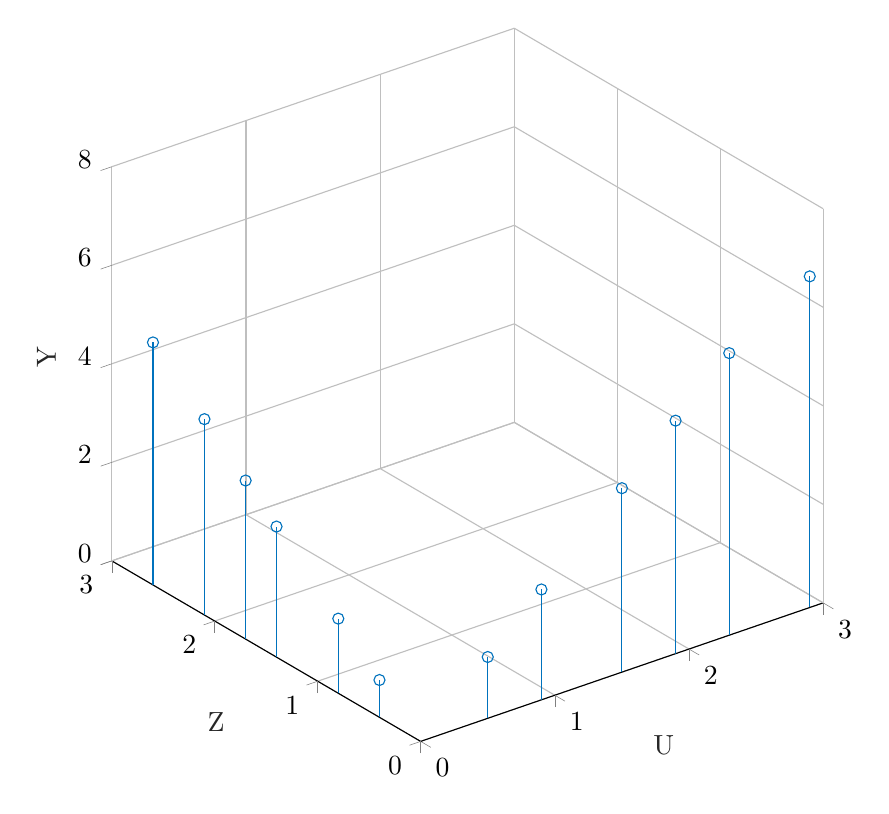
\begin{tikzpicture}

\begin{axis}[%
width=3.557in,
height=3.566in,
at={(0.597in,0.481in)},
scale only axis,
xmin=0,
xmax=3,
tick align=outside,
xlabel style={font=\color{white!15!black}},
xlabel={U},
ymin=0,
ymax=3,
ylabel style={font=\color{white!15!black}},
ylabel={Z},
zmin=0,
zmax=8,
zlabel style={font=\color{white!15!black}},
zlabel={Y},
view={-37.5}{30},
axis background/.style={fill=white},
title style={font=\bfseries},
title={ },
axis x line*=bottom,
axis y line*=left,
axis z line*=left,
xmajorgrids,
ymajorgrids,
zmajorgrids,
legend style={at={(1.03,1)}, anchor=north west, legend cell align=left, align=left, draw=white!15!black}
]
\addplot3 [ycomb, color=mycolor1, mark=o, mark options={solid, mycolor1}]
 table[row sep=crcr] {%
0.5	0	1.2446137691799\\
0.9	0	2.24030478452387\\
1.5	0	3.73384130753969\\
1.9	0	4.7295323228835\\
2.3	0	5.72522333822748\\
2.9	0	6.72091435357146\\
0	0.4	0.757307407029722\\
0	0.8	1.51461481405944\\
0	1.4	2.65057592460404\\
0	1.7	3.21855647987624\\
0	2.1	3.97586388690592\\
0	2.6	4.92249814569311\\
};

\end{axis}
\end{tikzpicture}%
	\label{sp}
\end{figure}

\begin{figure}
	\centering
	\caption{Charakterystyka statyczna - $Y(U)$}
	% This file was created by matlab2tikz.
%
\definecolor{mycolor1}{rgb}{0.00000,0.44700,0.74100}%
%
\begin{tikzpicture}

\begin{axis}[%
width=4.521in,
height=3.566in,
at={(0.758in,0.481in)},
scale only axis,
xmin=0.5,
xmax=3,
xlabel style={font=\color{white!15!black}},
xlabel={U},
ymin=0,
ymax=7,
ylabel style={font=\color{white!15!black}},
ylabel={Y},
axis background/.style={fill=white},
title style={font=\bfseries},
title={ },
legend style={legend cell align=left, align=left, draw=white!15!black}
]
\addplot[ycomb, color=mycolor1, mark=o, mark options={solid, mycolor1}] table[row sep=crcr] {%
0.5	1.2446137691799\\
0.9	2.24030478452387\\
1.5	3.73384130753969\\
1.9	4.7295323228835\\
2.3	5.72522333822748\\
2.9	6.72091435357146\\
};
\addplot[forget plot, color=white!15!black] table[row sep=crcr] {%
0.5	0\\
3	0\\
};


\end{axis}
\end{tikzpicture}%
	\label{spu}
\end{figure}

\begin{figure}
	\centering
	\caption{Charakterystyka statyczna - $Y(Z)$}
	% This file was created by matlab2tikz.
%
\definecolor{mycolor1}{rgb}{0.00000,0.44700,0.74100}%
%
\begin{tikzpicture}

\begin{axis}[%
width=4.521in,
height=3.566in,
at={(0.758in,0.481in)},
scale only axis,
xmin=0,
xmax=3,
xlabel style={font=\color{white!15!black}},
xlabel={Z},
ymin=0,
ymax=5,
ylabel style={font=\color{white!15!black}},
ylabel={Y},
axis background/.style={fill=white},
title style={font=\bfseries},
title={ },
legend style={legend cell align=left, align=left, draw=white!15!black}
]
\addplot[ycomb, color=mycolor1, mark=o, mark options={solid, mycolor1}] table[row sep=crcr] {%
0.4	0.757307407029722\\
0.8	1.51461481405944\\
1.4	2.65057592460404\\
1.7	3.21855647987624\\
2.1	3.97586388690592\\
2.6	4.92249814569311\\
};
\addplot[forget plot, color=white!15!black] table[row sep=crcr] {%
0	0\\
3	0\\
};


\end{axis}
\end{tikzpicture}%
	\label{spz}
\end{figure}

Na pierwszy rzut oka widać, że charakterystyki są liniowe, tzn. wartości $Y(U)$ i $Y(Z)$ ustalają się w przybliżeniu na linii prostej, za takie też będą traktowane w dalszych rozważaniach.

\section{Określenie wzmocnienia statycznego}
Na podstawie tej charakterystyki można obliczyć wzmocnienia statyczne obu torów procesu. Definiuje się je jako
\begin{equation}
K_U=\frac{\Delta Y}{\Delta U}, K_Z=\frac{\Delta Y}{\Delta Z}
\end{equation}
Pary parametrów $\Delta Y$ i $\Delta U$ oraz $\Delta Y$ i $\Delta Z$ są stałe dla dowolnie wybranych punktów na wykresach $Y(U)$ i $Y(Z)$, ponieważ charakterystyka jest liniowa. Należy więc wybrać dowolne punkty $(U_i, Y_i)$ i $(U_j, Y_j)$ oraz $(Z_i, Y_i)$ i $(Z_j, Y_j)$ i na ich podstawie obliczyć wzmocnienia statyczne $K_U$ i $K_Z$. Wyniki:
\begin{equation}
K_U=\num{2.49}, K_Z=\num{1.89}
\end{equation}